\chapter{Niet-Programmeerbare Processoren}
\chapterquote{We accepteren nu het feit dat leren een levenslang proces is om op de hoogte te blijven van veranderingen. En de meest urgente taak is mensen te leren hoe te leren.}{Peter F. Drucker, Amerikaans management consultant en auteur (1909-)}
\begin{chapterintro}
In de twee vorige hoofdstukken hebben we componenten gebouwd met een beperkte functionaliteit. De combinatorische schakelingen laten ons toe om schakelingen te ontwerpen die een rekenkundige operatie uitvoeren, maar we hebben geen geheugen beschikbaar om tussenresultaten in op te slaan. Het hoofdstuk over sequenti\"ele schakelingen maakt het mogelijk om schakelingen te ontwerpen met een geheugen. De meeste problemen hebben echter zeer grote toestandsruimtes (een 32-bit getal heeft meer dan vier miljard toestanden). Daarom volstaan de methodes uit dit hoofdstuk niet om een component te ontwikkelen die iets functioneel doet. Daarvoor zullen we methodes op een hoger niveau introduceren, dat van een niet-programmeerbare processor. Een niet programmeerbare processor voert een algoritme uit die op voorhand gekend is. Hierdoor kunnen we optimaal gebruik maken van de hardware en zoveel mogelijk instructies tegelijk uitvoeren. Het nadeel is dat eenmaal de processor geproduceerd is, we geen andere problemen met het component kunnen uitvoeren.
\end{chapterintro}
\minitoc[n]
\section{De Niet-Programmeerbare Processor}
Alvorens we de bouw van zo'n processor verder uitwerken, dienen we eerst enkele concepten te formaliseren. Allereerst ontleden we in deze sectie uit welke delen zo'n processor is opgebouwd. Vervolgens zullen we in sectie \ref{s:descriptionFSMD} een methode ontwikkelen om een algoritme formeel weer te geven. Deze beschrijving zal toelaten het algoritme later om te zetten naar een processor. In sectie \ref{s:memoryFSMD} ten slotte zullen we extra geheugencomponenten introduceren die we nodig zullen hebben bij de bouw van een processor.
\subsection{Algemene Structuur}
Een \termen{Niet-programmeerbare processor}, ofwel \termen{Finite State Machine with Data path (FSMD)} bestaat grofweg uit twee delen:
\begin{itemize}
 \item Een \termen{datapad}: een component die bewerkingen (rekenkundig, aritmetisch,...) uitvoert en de resultaten opslaat in tijdelijk geheugen.
 \item Een \termen{controller}: een component die het datapad aanstuurt. Het zegt welke actie op welk moment moet ondernomen worden.
\end{itemize}
In dit hoofdstuk is de controller niet programmeerbaar. Dat wil zeggen dat de controller telkens hetzelfde programma uitvoert. Dit betekent echter niet dat er een vaste cyclus in de controller zit. De controller kan afhankelijk van de waarden die in de geheugens van het datapad zitten, of van ingangen van de processor beslissen om andere acties te ondernemen. Een controller is dus een sequenti\"ele schakeling ofwel finite state machine. De synthese van een finite state machine werd in het hoofdstuk \ref{ch:SeqComp} reeds besproken. Uiteraard zullen we de karakteristieken die eigen zijn aan controllers in dit hoofdstuk bespreken.
\paragraph{}
Het spreekt voor zich dat de controller en het datapad continu data met elkaar uitwisselen. Enerzijds geeft de controller instructies aan het datapad. De groep signalen waarmee een controller een datapad aanstuurt noemen we het ``\termen{instructiewoord}'' ofwel ``\termen{controle-signalen}''. Anderzijds zullen de instructies vaak afhangen van de toestand van variabelen opgeslagen in het datapad. De verzameling van signalen die het datapad over zijn variabelen doorstuurt naar de controller noemen we ``\termen{statussignalen}''.
\paragraph{}
Een processor voert operaties uit op data. Deze data moet op de een of andere manier ingelezen worden in de processor. De verzameling ingangen waarmee we data vanuit de omgeving in het datapad injecteren noemen we de ``\termen{data-ingangen}''. Verder zullen we vaak ook informatie aan de controller moeten meedelen: we denken bijvoorbeeld aan een signaal die actief wordt wanneer alle data ingelezen is, en het algoritme kan uitgevoerd worden. Deze signalen noemen we ``\termen{controle-ingangen}''. Daarnaast willen we ook de resultaten kunnen uitlezen. Hiervoor voorzien we een reeks signalen vanuit het datapad, deze signalen noemen we ``\termen{data-uitgangen}''. Tot slot zijn we soms ook ge\"interesseerd in de toestand van het algoritme. We zullen bijvoorbeeld enkel data uitlezen indien het algoritme afgelopen is. De controller kan informatie over het algoritme naar buiten brengen via ``\termen{controle-uitgangen}''. De verschillende informatiestromen tussen het datapad en de controller en de processor en zijn omgeving beschrijven we op figuur \ref{fig:processorInformationStreams}.
\begin{figure}[hbt]
\centering
\subfigure[Processor]{
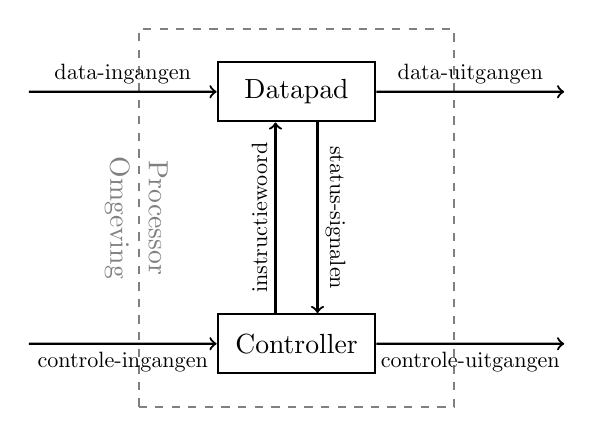
\begin{tikzpicture}[scale=0.8]
\draw[gray,dashed,thick] (-2.5,-3) rectangle (2.5,3);
\draw (-2.5,0) node[rotate=-90,gray,anchor=south]{Processor};
\draw (-2.5,0) node[rotate=-90,gray,anchor=north]{Omgeving};
\node[rectangle,thick,draw=black,minimum width=2 cm,minimum height=0.75 cm] (D) at (0,2) {Datapad};
\node[rectangle,thick,draw=black,minimum width=2 cm,minimum height=0.75 cm] (C) at (0,-2) {Controller};
\draw[->,thick] (D.south -| 0.3333,0) to node[midway,sloped,above,scale=0.8]{status-signalen} (C.north -| 0.3333,0);
\draw[->,thick] (C.north -| -0.3333,0) to node[midway,sloped,above,scale=0.8]{instructiewoord} (D.south -| -0.3333,0);
\draw[<-,thick] (C.west) to node[below,midway,scale=0.8]{controle-ingangen} (-4.25,-2);
\draw[->,thick] (C.east) to node[below,midway,scale=0.8]{controle-uitgangen} (4.25,-2);
\draw[<-,thick] (D.west) to node[above,midway,scale=0.8]{data-ingangen} (-4.25,2);
\draw[->,thick] (D.east) to node[above,midway,scale=0.8]{data-uitgangen} (4.25,2);
\end{tikzpicture}
\label{fig:processorInformationStreams}}
\subfigure[Datapad]{
\begin{tikzpicture}[scale=0.8]
\draw[gray,dashed,thick] (-3.5,-3) rectangle (3.5,3);
\draw (-3.5,1.3) node[rotate=-90,gray,anchor=south]{Datapad};
\draw (-3.5,1.3) node[rotate=-90,gray,anchor=north]{Omgeving};
\node[rectangle,thick,draw=black,minimum width=2 cm] (T) at (0,1.25) {Tijdelijk geheugen};
\node[trapezium,thick,draw=black] (O) at (0,0) {Operatorverbindingen};
\node[rectangle,thick,draw=black,minimum width=2 cm] (F) at (0,-1.25) {Functionele eenheden};
\node[minimum width=2 cm] (RA) at (0,-2.5) {Resultaatverbindingen};
\node[minimum width=2 cm,white] (RB) at (0,2.5) {Resultaatverbindingen};
\draw[thick] (RA.north west) -- (O.bottom left corner |- RA.south) -- (RA.south east) -- ++(1,0) |- (RB.north west) -- (RB.south -| O.bottom left corner) -- (RB.south east) -- ++(0.5,0) |- (RA.north west);
\draw[thick,->] (RB) -- (T);
\draw[thick,->] (T) -- (O);
\draw[thick,->] (O) -- (F);
\draw[thick,->] (F) -- (RA);
\draw[<-,thick] (RA.west -| O.west) -- ++(-3,0);
\draw[<-,thick] (RB.west -| O.west) -- ++(-3,0);
\draw (-4,0) node[scale=0.8,anchor=south]{instructiewoord};
\draw (-4,-2.5) node[scale=0.8,anchor=south]{instructiewoord};
\draw (-4,2.5) node[scale=0.8,anchor=south]{externe-ingangen};
\draw (1.75,-3.5) node[scale=0.8,anchor=south]{externe-uitgangen};
\draw[<-,thick] (O.west) -- ++(-3,0);
\draw[->,thick] (RA) |- ++(3.5,-1);
\end{tikzpicture}
\label{fig:datapadInformationStreams}}
\caption{Opbouw van een processor en datapad.}
\end{figure}
\paragraph{}
Door de controle-ingangen wordt de definitie van ``niet-programmeerbaar'' natuurlijk vaag. We zouden immers het toestandswoord van de controller in grote mate laten afhangen van de invoer die de controle-ingangen. Hierdoor kunnen we de processor toch programmeren. Het onderscheid is dan ook eerder een common-sense.
\subsection{Het Datapad}
Zoals we reeds hebben vermeld, kunnen we een controller modelleren als een eindige toestandsautomaat ofwel finite state machine. Een datapad daarentegen bestaat uit verschillende componenten:
\begin{itemize}
 \item \termen{Functionele Eenheden} ofwel \termen{Functional Units (FU)}: dit zijn schakelingen die berekeningen en aritmetisch operaties uitvoeren. Dit zijn dus de componenten die we in hoofdstuk \ref{ch:combinatoric} hebben besproken: optellers, ALU, schuifoperator,... Uiteraard kunnen we ook zelf functionele eenheden bouwen op de manier die we gezien hebben.
 \item \termen{Tijdelijke geheugens}: dit zijn componenten die de waarden waarop we bewerkingen uitvoeren voor enkele klokcycli kunnen vasthouden. Dit zijn bijvoorbeeld de registerbanken en RAM die we in sectie \ref{s:memoryFSMD} zullen invoeren. Het zijn groepen van flipflops die ons toelaten om op een hoger niveau te redeneren.
 \item \termen{Verbindingen}: de tijdelijke geheugens en de functionele eenheden wisselen informatie uit. Daarom hebben we twee types verbindingen nodig:
 \begin{itemize}
  \item \termen{Operandverbindingen}: dit zijn verbindingen die de waardes van de tijdelijke geheugens overbrengen als operanden van de functionele eenheden. De waarde van een register kan op die manier bijvoorbeeld gebruikt worden bij een optelling.
  \item \termen{Resultaatverbindingen}: het is de bedoeling dat de resultaten vervolgens in een tijdelijk geheugen opgeslagen worden. Resultaatverbindingen transporteren de resultaten van de functionele eenheden terug naar de tijdelijke geheugens. Sommige uitvoer kan ook weggeschreven worden naar de data-uitgangen. Ook de invoer van de data-ingangen wordt door deze verbindingen verwerkt.
 \end{itemize}
 Het spreekt voor zich dat de verbindingen beslissen welke geheugens als operanden en resultaatgeheugens dienen. Daarom zullen we ze implementeren als bussen met multiplexers en 3-state buffers. Deze bussen zullen dan worden aangestuurd door de controller.
\end{itemize}
Dit concept beschrijven we op figuur \ref{fig:datapadInformationStreams}.
\paragraph{}
In het datapad doen we dan ook niets anders dan waardes uit het tijdelijke geheugen inlezen, er een operatie van een functionele eenheid op uitvoeren en vervolgens in een tijdelijk geheugen plaatsen. Dit proces noemen we ook wel de ``\termen{registertransfer}'' en formaliseren we als:
\begin{equation}
\mbox{register}_a\leftarrow\mbox{FU}_a\left(\mbox{register}_{a_1},\mbox{register}_{a_1},\mbox{register}_{a_2},\ldots,\mbox{register}_{a_n}\right)
\end{equation}
In het eerste hoofdstuk hebben we reeds vermeld dat we schakelingen bij het bouwen van een processor beschrijven op registertransfer-niveau. Dit betekent dat we bijvoorbeeld abstractie zullen maken van flipflops en zullen werken met registers. Ook zullen we details als het aantal bits die een opteller nodig heeft verwaarlozen. Deze nieuwe notatiestijl zullen we geleidelijk invoeren.
\section{Formeel Beschrijven van een Algoritme}
\label{s:descriptionFSMD}
Alvorens we een processor kunnen bouwen die een algoritme uitvoert, moeten we eerst een formeel algoritme kunnen opstellen. Dit algoritme vertrekt altijd vanuit een probleemstelling. Hoe we een probleemstelling omzetten naar een algoritme behoort niet tot de inhoud van deze cursus\footnote{Het omzetten van een probleem in een algoritme is geen exacte wetenschap. Het is een vaardigheid die wel geoefend kan worden. Hiervoor bestaan er andere cursussen.}. We zullen altijd stellen dat het algoritme vooraf gekend moet zijn.
\subsection{Leidend Voorbeeld: Deler}
Als leidend voorbeeld doorheen dit hoofdstuk zullen we een processor bouwen die natuurlijke getallen kan delen. Uiteraard zouden we hiervoor een combinatorische schakeling kunnen bouwen. We zullen echter een algoritme beschouwen om de berekening te maken. De processor heeft 2 4-bit ingangen die het deeltal en de deler inlezen. Verder bevat het ook een controle-ingang. Zolang we een laag signaal op de controle-ingang aanleggen betekent dit dat er geen correcte invoer op de data-ingangen staat. Pas wanneer we een hoog signaal aanleggen zal het algoritme dus een deling uitvoeren. Verder bevat de processor ook 2 4-bit uitgang om het quoti\"ent en de rest naar buiten te brengen, en een controle uitgang die hoog wordt op het moment dat het algoritme het quoti\"ent en de rest heeft berekend. Zolang de controle-uitgang dus laag is, is het algoritme nog bezig met de berekening. Verder zal de processor ook wachten totdat de controle-ingang eerst laag is geweest alvorens opnieuw te beginnen. We maken de assumptie dat de deler nooit gelijk is aan 0. Het algoritme die dan vervolgens het deeltal en de deler omzet in het quoti\"ent en rest staat op \algoref{alg:devisionFSMD}.
\begin{algorithm}[hbt]
\caption{Delen van twee $n$-bit getallen.}\label{alg:devisionFSMD}
\begin{algorithmic}[1]
\Function{Division}{$N,D$}
\State $Q\gets 0$
\State $R\gets 0$
\For{$I=n-1\mbox{ \textbf{to} }0$}
\State $R\gets R\shlcmd{}1$\Comment{Logische shift $R$ naar links over 1 positie}
\State $R\left[0\right]\gets N\left[n-1\right]$
\State $N\gets N\shlcmd{}1$\Comment{Logische shift $N$ naar links over 1 positie}
\State $Q\gets Q\shlcmd{}1$\Comment{Logische shift $Q$ naar links over 1 positie}
\If{$R\geq D$}
\State $R\gets R-D$
\State $Q\left[0\right]\gets 1$
\EndIf
\EndFor
\State \Return $\left(Q,R\right)$
\EndFunction
\end{algorithmic}
\end{algorithm}
We gaan niet in op de precieze werking van het algoritme. Indien we een index opvragen of zetten bij een variabele zoals $V\left[i\right]$ betekent dit dat we een operatie op de $i$-de bit uitvoeren. We tellen we van rechts naar links, $V[0]$ is dus de minst beduidende bit van $V$ die rechts staat in de encodering. Verder zullen we ook de subscript-notatie gebruiken wanneer we bits samen nemen. Zo betekent $v_2v_1w_2w_2v_2w_1$ dat we een getal samenstellen uit de eerste twee bits van $V$, gevolgd door de eerste en de derde bit van $W$, daarna volgen nog de derde bit van $V$ en de tweede bit van $W$. Dit algoritme is echter niet geschikt voor een processor. Een processor voert immers continu het programma uit. Bovendien wordt hier niet gewacht tot er invoer op de data-ingangen staat. Een laatste opmerking is dat we geen berekeningen op invoer kunnen uitvoeren. Anders zouden we immers de uitgangen van functionele eenheden met de ingangen van de processor verbinden. Daarom dienen we variabelen te introduceren die we $X$, $Y$ en $Z$. Daarom zullen we het algoritme herschrijven\footnote{Strikt genomen is dit geen algoritme meer, vermits het nooit eindigt en er geen echt resultaat is. Een betere bewoording is waarschijnlijk procedure.}. We beschouwen hierbij de controle-ingang $ci$ en de controle-uitgang $co$. De herschreven procedure staat in \algoref{alg:devisionFSMDRev}.
\begin{algorithm}[hbt]
\caption{Procedure voor het delen van twee $4$-bit getallen.}\label{alg:devisionFSMDRev}
\begin{algorithmic}[1]
\Procedure{Division}{}
\While{true}
\Repeat\label{algl:s1start}
\State $co\gets 0$
\State $X\gets N$
\State $Y\gets 0$
\State $Z\gets 0$
\Until{$ci$}\label{algl:s1stop}
\For{$I=3\mbox{ \textbf{to} }0$}\label{algl:s2start}
\State $Z\gets Z\shlcmd{}1$\Comment{Logische shift $Z$ naar links over 1 positie}
\State $Z\left[0\right]\gets X\left[3\right]$
\State $X\gets X\shlcmd{}1$\Comment{Logische shift $X$ naar links over 1 positie}
\State $Y\gets Y\shlcmd{}1$\Comment{Logische shift $Y$ naar links over 1 positie}
\If{$Z\geq D$}\label{algl:devisionFSMDComp}
\State $Z\gets Z-D$\label{algl:devisionFSMDSub}
\State $Y\left[0\right]\gets 1$
\EndIf
\EndFor\label{algl:s2stop}
\Repeat\label{algl:s3start}
\State $co\gets 1$
\State $Q\gets Y$
\State $R\gets Z$
\Until{$\neg ci$}\label{algl:s3stop}
\EndWhile
\EndProcedure
\end{algorithmic}
\end{algorithm}
\subsection{Toestandsbeschrijving}
Een eerste probleem dient zich aan hoe we de procedure omzetten in een reeks toestanden. De vraag is immers wat we in \'e\'en zo'n toestand zullen realiseren. Zo kunnen we \algoref{alg:devisionFSMDRev} uitvoeren en per instructie een nieuwe toestand bouwen. Als we echter het programma onder de loep nemen, zien we dat dit algoritme zich uitstekend leent om verschillende instructies samen uit te voeren. Allereerst voeren we in de \textbf{for}-lus hoofdzakelijke shift operaties uit. Deze shiftoperaties vinden plaats over een vast aantal posities. We dienen dus helemaal geen schuifoperator te implementeren, en kunnen eenvoudigweg schuiven met verbindingen. Vervolgens doen we ook aan bitmanipulaties. Omdat deze bitmanipulaties opnieuw op vaste plaatsen plaatsvinden kunnen we dit realiseren met behulp van verbindingen. De enige twee aspecten die enige logica vereisen is de test of $Z\geq D$ is (lijn \ref{algl:devisionFSMDComp}), en het eventueel aftrekken van $D$ uit $Z$ (lijn \ref{algl:devisionFSMDSub}). Daarnaast moeten we tijdens de uitvoer van de \textbf{for} lus ook controleren of $I\geq 0$. In dat geval dienen we immers nogmaals de for-lus uit te voeren. We kunnen dit echter controleren met een simpele OR-poort die alle bits van $I$ samenneemt. Indien minstens \'e\'en van de bits een 1 is, zal de OR-lus een 1 teruggeven, en dienen we dus nog een cyclus uit te voeren. Dit leidt ertoe dat we ons algoritme in drie toestanden opdelen:
\begin{enumerate}
 \item $S_0$: inlezen van invoer, initialiseren van variabelen en wachten totdat $ci$ hoog wordt (lijnen \ref{algl:s1start}-\ref{algl:s1stop}).
 \item $S_1$: uitvoeren van een cyclus van de \textbf{for} lus en $I$ met 1 verlagen (lijnen \ref{algl:s2start}-\ref{algl:s2stop}).
 \item $S_2$: resultaten op de uitgang plaatsen en wachten tot $ci$ laag wordt (lijnen \ref{algl:s3start}-\ref{algl:s3stop}).
\end{enumerate}
\subsection{Toestand-Actie Tabel}
Nu we de toestanden hebben vastgesteld kunnen we het algoritme verder formaliseren. Dit zouden we kunnen doen met een grafische voorstelling zoals we gedaan hebben met een eindige toestandsautomaat. Het probleem is dat een rij in het toestandsdiagram niet enkel de voorwaarden en eventuele uitgangen bevat, daarnaast dient het ook nog de acties die door het datapad moeten worden uitgevoerd weer te geven. Dit zou leiden tot een complex en chaotisch diagram. Daarom verkiezen we een tabel: de ``\termen{Toestand-Actie Tabel}''. De tabel bestaat grofweg uit drie gedeeltes:
\begin{itemize}
 \item de huidige toestand: de huidige toestand waarin de controller zich bevindt.
 \item Een toestandsgedeelte: die we kunnen vergelijken met de toestandstabel van een eindige toestandsautomaat. De tabel bevat volgende kolommen:
 \begin{itemize}
  \item condities (afhankelijk van controle- en status-signalen)
  \item de volgende toestand
  \item de uitvoer (van eventuele controle-uitgangen).
 \end{itemize}
 \item een controle-actie gedeelte. Dit gedeelte bevat twee kolommen:
 \begin{itemize}
  \item conditie: een set voorwaarden wanneer een bepaalde set acties (gespecificeerd in de volgende kolom) moet worden uitgevoerd.
  \item actie: afhankelijk van de conditie welke opdrachten uitgevoerd worden op de variabelen in een klokcyclus.
 \end{itemize}
\end{itemize}
Tabel \ref{tbl:stateActionTableRunningExample} toont de toestand-actie tabel van \algoref{alg:devisionFSMDRev}. Een belangrijke opmerking is dat het onderverdelen van toestanden in condities bij het toestandsgedeelte niet verder loopt bij het onderverdelen van diezelfde toestand in het controle-actie gedeelte. Dit betekent dus dat de conditie bij de volgende toestand niet de conditie bij de controle- en datapad-acties impliceert en omgekeerd. Concreet betekent dit dus dat indien $I>0$, dit niet betekent dat $z_2z_1z_0x_3<D$ of dat we de bijbehorende datapad-acties moeten uitvoeren. Het toestandsgedeelte en het controle-actie gedeelte zijn dus onafhankelijk en zijn enkel afhankelijk van de huidige toestand.
\begin{table}[hbt]
\centering
\begin{tabular}{c!{\vrule width 1pt}c|c|c!{\vrule width 1pt}c|c}
Huidige&\multicolumn{2}{c|}{Volgende toestand}&Uit-&\multicolumn{2}{c}{Controle- \& datapad-acties}\\
Toestand&Conditie&Toestand&gang&Conditie&Acties\\\noalign{\hrule height 1pt}
\multirow{4}{*}{$S_0$}&\multirow{2}{*}{$ci=0$}&\multirow{2}{*}{$S_0$}&\multirow{2}{*}{$co=0$}&&$X\gets N$\\
&&&&&$Y\gets 0$\\\cline{2-4}
&\multirow{2}{*}{$ci=1$}&\multirow{2}{*}{$S_1$}&\multirow{2}{*}{$co=0$}&&$Z\gets 0$\\
&&&&&$I\gets 3$\\\noalign{\hrule height 1pt}
\multirow{8}{*}{$S_1$}&\multirow{4}{*}{$I>0$}&\multirow{4}{*}{$S_1$}&\multirow{4}{*}{$co=0$}&\multirow{4}{*}{$z_2z_1z_0x_3<D$}&$Z\gets z_2z_1z_0x_3$\\
&&&&&$X\gets X\shlcmd 1$\\
&&&&&$Y\gets Y\shlcmd 1$\\
&&&&&$I\gets I-1$\\\cline{2-6}
&\multirow{4}{*}{$I=0$}&\multirow{4}{*}{$S_2$}&\multirow{4}{*}{$co=0$}&\multirow{4}{*}{$z_2z_1z_0x_3\geq D$}&$Z\gets z_2z_1z_0x_3-D$\\
&&&&&$X\gets X\shlcmd 1$\\
&&&&&$Y\gets y_2y_1y_01$\\
&&&&&$I\gets I-1$\\\noalign{\hrule height 1pt}
\multirow{6}{*}{$S_2$}&\multirow{3}{*}{$ci=0$}&\multirow{3}{*}{$S_0$}&$co=1$&&\\
&&&$Q=Y$&&\\
&&&$R=Z$&&\\\cline{2-4}
&\multirow{3}{*}{$ci=1$}&\multirow{3}{*}{$S_2$}&$co=1$&&\\
&&&$Q=Y$&&\\
&&&$R=Z$&&\\
\end{tabular}
\caption{Toestand-actie tabel van het leidend voorbeeld.}
\label{tbl:stateActionTableRunningExample}
\end{table}
\paragraph{Simulatie}Om ons meer vertrouwd te maken met het concept van een toestand-actie tabel zullen we een deling simuleren met behulp van de tabel. We zullen $N=12$ delen door $D=7$ op de processor en stap per stap kijken wat er verandert. Dit doen we met behulp van tabel \ref{tbl:stateActionTableRunningExampleSim}. Omdat we met bitoperaties werken zullen we alle variabelen in de tabel in binaire notatie zetten.
\begin{table}[hbt]
\centering
\begin{tabular}{c|c|c|c}
Toestand&Voldane Condities&Acties&Uitvoer\\\hline
\multirow{4}{*}{$S_0$}&\multirow{4}{*}{$ci=1$}&$X\gets N=1100$&\multirow{4}{*}{$co=0$}\\
&&$Y\gets0000$&\\
&&$Z\gets0000$&\\
&&$I\gets11$&\\\hline

\multirow{4}{*}{$S_1$}&\multirow{2}{*}{$I=11>00$}&$Z\gets z_2z_1z_0x_3=0001$&\multirow{4}{*}{$co=0$}\\
&&$X\gets X\shlcmd{} 1=1000$&\\
&\multirow{2}{*}{$z_2z_1z_0x_3=0001<D=0101$}&$Y\gets Y\shlcmd{} 1=0000$&\\
&&$I\gets I-1=10$&\\\hline

\multirow{4}{*}{$S_1$}&\multirow{2}{*}{$I=10>00$}&$Z\gets z_2z_1z_0x_3=0011$&\multirow{4}{*}{$co=0$}\\
&&$X\gets X\shlcmd{} 1=0000$&\\
&\multirow{2}{*}{$z_2z_1z_0x_3=0011<D=0101$}&$Y\gets Y\shlcmd{} 1=0000$&\\
&&$I\gets I-1=01$&\\\hline

\multirow{4}{*}{$S_1$}&\multirow{2}{*}{$I=01>00$}&$Z\gets z_2z_1z_0x_3-D=0001$&\multirow{4}{*}{$co=0$}\\
&&$X\gets X\shlcmd{} 1=0000$&\\
&\multirow{2}{*}{$z_2z_1z_0x_3=0110\geq D=0101$}&$Y\gets y_2y_1y_01=0001$&\\
&&$I\gets I-1=00$&\\\hline

\multirow{4}{*}{$S_1$}&\multirow{2}{*}{$I=00$}&$Z\gets z_2z_1z_0x_3=0010$&\multirow{4}{*}{$co=0$}\\
&&$X\gets X\shlcmd{} 1=0000$&\\
&\multirow{2}{*}{$z_2z_1z_0x_3=0010<D=0101$}&$Y\gets Y\shlcmd{} 1=0010$&\\
&&$I\gets I-1=11$&\\\hline

\multirow{3}{*}{$S_2$}&\multirow{3}{*}{$ci=0$}&&$co=1$\\
&&&$Q=Y=0010$\\
&&&$R=Z=0010$\\
\end{tabular}
\caption{Simulatie van het algoritme met behulp van de toestand-actie tabel (tabel \ref{tbl:stateActionTableRunningExample}).}
\label{tbl:stateActionTableRunningExampleSim}
\end{table}
We stellen dat vanaf dat we de simulatie beginnen, reeds de data reeds op de ingangen van de processor aangelegd staat. Bijgevolg is $ci=1$, $N=1100$ en $D=0101$. We maken verder ook een assumptie dat $X$, $Y$ en $Z$ 4-bit geheugens zijn, dit is redelijk vermits we uitsluitend bits in dit bereik gebruiken, en we geen schuifoperaties naar rechts uitvoeren waardoor hogere bits in het bereik zouden komen te liggen. $I$ is een 2-bit geheugen vermits het uitsluitend waardes tussen 0 en 3 moet aannemen. Initieel vertrekt de processor vanuit toestand $S_0$ we zien op die toestand-actie tabel dat in toestand $S_0$ de ingangen in de geheugens worden ingelezen. Vermits er data op de ingangen staat, krijgt $X$ de waarde van de teller $N=1100$. De overige variabelen worden ge\"initialiseerd zoals beschreven staat in de toestand-actie tabel. Omdat $ci=1$ kunnen we afleiden dat de volgende toestand $S_1$ is. Verder specificeert de tabel ook dat we een laag signaal op de controle-uitgang moeten aanleggen (momenteel staat er immers geen uitkomst op de uitgangen). In de volgende stap bevinden we ons in toestand $S_1$. We evalueren eerst de verschillende condities ??.
\subsection{ASM-Schema}
Zoals reeds gezegd is de visualisatie van een eindige toestandsautomaat niet toereikend om een algoritme weer te geven. Een grafisch voorstelling die we wel kunnen gebruiken is een ``\termen{Algorithmic-State-Machine Chart}'' ofwel ``\termen{ASM-schema}''. Een ASM-schema lijkt op een flow-chart en bestaat drie verschillende soorten ``\termen{ASM-elementen}'':
\begin{itemize}
 \item \termen{Toestandskader} ofwel \termen{state box}: dit is een set niet-conditionele toekenning. We stellen een toestandskader voor door middel van een rechthoek waarin we de toekenningen schrijven. De toekenningen in \'e\'en toestandskader worden parallel uitgevoerd. Figuur \ref{fig:asmElementState} toont een voorbeeld van een toestandskader.
 \item \termen{Beslissingskader} ofwel \termen{decision box}: dit is de voorstelling van een bepaalde conditie. Een conditie wordt voorgesteld met behulp van een ruit, waarin de conditie wordt geschreven. Vanuit een beslissingskader vertrekken er twee pijlen: voor het geval waarin de voorwaarde waar of vals is. Figuur \ref{fig:asmElementDecision} toont een voorbeeld van een beslissingskader.
 \item \termen{Conditioneel kader} ofwel \termen{conditional box}: Dit is een toestandskader die enkel onder voorwaarden gespecificeerd door een beslissingskader worden uitgevoerd. Ook deze toekenningen worden in parallel uitgevoerd. Men stelt een conditioneel kader voor als een rechthoek met afgeronde hoeken. Figuur \ref{fig:asmElementConditional} toont een voorbeeld van een conditioneel kader.
\end{itemize}
\begin{figure}[hbt]
\centering
\subfigure[Toestandskader]{
\begin{tikzpicture}
\node[asmS] (S) at (0,0) {$\begin{array}{c}\mbox{niet conditioneel commando 1}\\\mbox{niet conditioneel commando 2}\\\cdots\\\mbox{niet conditioneel commando $n$}\end{array}$};
\draw[<-] (S) -- ++(0,1.5) node[anchor=south]{in};
\draw[->] (S) -- ++(0,-1.5) node[anchor=north]{uit};
\end{tikzpicture}
\label{fig:asmElementState}
}
\subfigure[Beslissingskader]{
\begin{tikzpicture}
\node[asmD] (D) at (0,0) {test};
\draw[<-] (D) -- ++(0,1.5) node[anchor=south]{in};
\draw[->] (D) -| ++(-1.75,-1.5) node[anchor=north]{uit 1};
\draw[->] (D) -| ++(1.75,-1.5) node[anchor=north]{uit 2};
\draw (-1.75,0) node[anchor=south west,scale=0.75]{[True]};
\draw (1.75,0) node[anchor=south east,scale=0.75]{[False]};
\end{tikzpicture}
\label{fig:asmElementDecision}
}
\subfigure[Conditioneel kader]{
\begin{tikzpicture}
\node[asmC] (C) at (0,0) {$\begin{array}{c}\mbox{conditioneel commando 1}\\\mbox{conditioneel commando 2}\\\cdots\\\mbox{conditioneel commando $n$}\end{array}$};
\draw[<-] (C) -- ++(0,1.5) node[anchor=south]{in};
\draw[->] (C) -- ++(0,-1.5) node[anchor=north]{uit};
\end{tikzpicture}
\label{fig:asmElementConditional}
}
\caption{Voorstelling van de verschillende ASM-elementen}
\label{fig:asmElementsEnum}
\end{figure}
Deze ASM-elementen worden gegroepeerd in een ``\termen{ASM-blok}''. Al deze elementen worden dan in \'e\'en klokcyclus uitgevoerd. Hierdoor voorzien we per toestand in de Toestand-Actie tabel een ASM-blok. Het blok zelf moet dan specificeren wat er in de toestand gebeurt. We zullen dit component voorstellen met behulp van een vierkant met streepjeslijnen. Vermits alle acties in \'e\'en klokflank uitgevoerd worden, bevat elk ASM-blok exact \'e\'en toestandskader. Dit toestandskader bevat dan alle acties die onafhankelijk van condities in die toestand worden uitgevoerd. Indien er geen onafhankelijke operaties zijn, is het vierkant leeg.
\begin{figure}[hbt]
\centering
\begin{tikzpicture}
\def\ds{6};
\def\di{1.75};
\def\dy{-2};
\def\offset{1};
\node[asmS] (S1S) at (0,0) {$\begin{array}{c}X\gets N\\Y\gets 0\\Z\gets 0\\I\gets 3\\co=0\end{array}$};
\node[asmD] (S1D) at (0,\dy) {$ci=0$};
\draw[->] (S1S) -- (S1D);
\draw[->] (S1D) -| (-\di,0) -- (S1S);
\setTrueFalseLabels{S1D};

\node[asmS] (S2S) at (\ds,0) {$\begin{array}{c}X\gets N\\I\gets I-1\\co=0\end{array}$};
\node[asmD] (S2D1) at (\ds,\dy) {$z_2z_1z_0x_3<D$};
\draw[->] (S2S) -- (S2D1);
\node[asmC] (S2C1) at (\ds-\di,2*\dy) {$\begin{array}{c}Z\gets z_2z_1z_0x_3\\Y\gets Y\shlcmd{} 1\end{array}$};
\draw[->] (S2D1) -| (S2C1);
\node[asmC] (S2C2) at (\ds+\di,2*\dy) {$\begin{array}{c}Z\gets z_2z_1z_0x_3-D\\Y\gets y_2y_1y_01\end{array}$};
\draw[->] (S2D1) -| (S2C2);
\draw (S2C1) |- (\ds,2.5*\dy) -| (S2C2);
\node[asmD] (S2D2) at (\ds,3*\dy) {$I>0$};
\draw[->] (\ds,2.5*\dy) -- (S2D2);
\draw[->] (S1D) -| (\di,\offset) -| (S2S);
\draw[->] (S2D2) -| (\ds-2*\di,0) -- (S2S);
\setTrueFalseLabels{S2D1};
\setTrueFalseLabels{S2D2};

\node[asmS] (S3S) at (2*\ds,0) {$\begin{array}{c}co=1\end{array}$};
\node[asmD] (S3D) at (2*\ds,\dy) {$ci=1$};
\draw[->] (S2D2) -| (\ds+2*\di,\offset) -| (S3S);
\draw[->] (S3S) -- (S3D);
\draw[->] (S3D) -| (2*\ds-\di,0) -- (S3S);
\draw[->] (S3D) -| (\di+2*\ds,1.5) -| (S1S);
\setTrueFalseLabels{S3D};
\begin{pgfonlayer}{background}
\node[asmB, fit=(S1S) (S1D)] {};
\node[asmB, fit=(S2S) (S2D1) (S2D2) (S2C1) (S2C2)] {};
\node[asmB, fit=(S3S) (S3D)] {};
\end{pgfonlayer}
\end{tikzpicture}
\caption{ASM-schema van het leidend voorbeeld.}
\end{figure}
\subsubsection{Traditionele Valkuilen}
\section{Geheugencomponenten}
\label{s:memoryFSMD}
\subsection{Registerbank}
\subsection{Random Access Memory (RAM)}
\subsection{Stack (LIFO: Last-In-First-Out)}
\subsection{Queue (FIFO: First-In-First-Out)}
\section{Synthese van een Niet-Programmeerbare Processor}
\label{s:syntheseFSMD}
\section{Tijdsgedrag}
\label{s:timeFSMD}